%!TEX program = xelatex
\documentclass[cn,hazy,blue,screen,14pt]{template}
\usepackage{tikz}
\title{学习笔记}

\author{}

%\version{0.00}
\date{\zhtoday}

\begin{document}

\maketitle
\newpage
\tableofcontents
\newpage

\section{算法}
\subsection{Morris traversal}

迭代,O(1)空间,修改叶结点的左右节点实现遍历。

中序:

根结点出发,记录当前节点。重复以下过程至当前节点为空:

1、若当前节点无左结点,输出并转移至右节点;

2、考虑当前节点的前驱节点,无右节点则将其右节点指向当前节点且当前节点左移,有右节点则当前节点变为其右节点,再将该节点的右节点还原为空,输出当前节点,当前节点右移。

\subsection{Brian Kernighan算法}
清除二进制最右边的1(number-1和number与运算)

\subsection{欧拉回路/通路}
定义:经过图中所有边一次且经过所有顶点的回路/通路\\

判定:

无向图G存在欧拉通路的充要条件是:

G为连通图,并且G仅有两个奇度结点(度数为奇数的顶点)或者无奇度结点。

有向图D存在欧拉通路的充要条件是:

D为有向图,D的基图连通,并且所有顶点的出度与入度都相等;或者除两个顶点外,其余顶点的出度与入度都相等,而这两个顶点中一个顶点的出度与入度之差为1,另一个顶点的出度与入度之差为-1。

\subsection{AVL tree}
\subsection{数位dp}
\subsection{lca}
\subsection{差分树}

\subsection{并查集}

按秩合并可撤销
\subsection{矩阵树定理}
\newpage

\section{软件}

\subsection{git}

安装:apt-get install git

设置:git config --global (user.name "", user.email"", core.editor vim, color.ui true)

初始化:git init

查看存档及变化信息:git log/status

跟踪文件:git add (filename/-A全选)(可编辑.gitignore)

存档:git commit

读档:git reset --hard (hash code)(清除所有新的记录)

分支:git branch;git checkout (-B修改输出至新分支) 分支名 


\newpage

\section{something}

注意数据范围

上取整:(a-1)/b+1



\subsection{\#if \#else \#endif}
c语言字符串常量写一起会拼接

gcc --verbose


\newpage
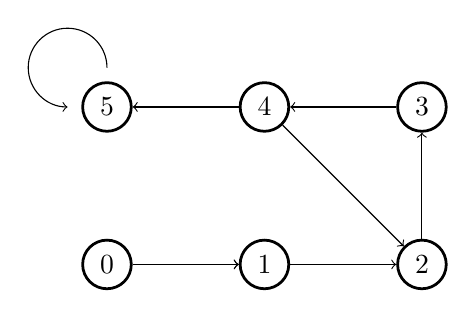
\begin{tikzpicture}
\node[circle, draw =black, line width=1pt] (a) at (0,0){0};
\node[circle, draw =black, line width=1pt] (b) at (2,0){1};
\node[circle, draw =black, line width=1pt] (c) at (4,0){2};
\node[circle, draw =black, line width=1pt] (d) at (4,2){3};
\node[circle, draw =black, line width=1pt] (e) at (2,2){4};
\node[circle, draw =black, line width=1pt] (f) at (0,2){5};
\draw [->] (a)--(b);
\draw [->] (b)--(c);
\draw [->] (c)--(d);
\draw [->] (d)--(e);
\draw [->] (e)--(f);
\draw [->] (e)--(c);
\draw [->] (a)--(b);
\draw [->] (0,2.5) arc (0:270:0.5);
\end{tikzpicture}

(0, x, x) -> (1, 0, x) -> (2, 0, 0) -> (3, 0, 1) -> (4, 1, 1) -> (2, 1, 1) -> (3, 1, 2) -> (4, 3, 2) -> (2, 3, 2) -> (3, 3, 3) -> (4, 6, 3) -> (2, 6, 3) -> ...... -> (2, 4851, 98) -> (3, 4851, 99) -> (4, 4950, 99) -> (2, 4950, 99) -> (3, 4950, 100) -> (4, 5050, 100) -> (5, 5050, 100) -> (5, 5050, 100)......



























\end{document}

